\section{Redes Neurais Convolucionais}
\label{cnn}

Dentre os tipos de rede de aprendizado profundo, a mais utilizada atualmente para trabalhar com visão computacional e processamento de imagens, de modo geral, e que possui valor notório para o trabalho com dados espaciais \citep{Goodfellow2016, ponti2018funciona, Ghosh2019}, destaca-se a denominada \textit{Convolutional Neural Networks}\citep{LeCun1999}, ou a célebre CNN, que tem esse nome por trabalhar com camadas convolucionais.

Evidencia-se que as CNNs são consideradas como estado-da-arte em algumas competições \cite{Parkhi2015}, assim como modelo bioinspirado de sucesso \cite{Goodfellow2016}, visto que esta simula pontos cerebrais responsáveis pela captura de impulsos visuais e outras propriedades que são capturadas pelo córtex visual, além de obter diferentes características que desenvolveram as operações de \textit{pooling} \cite{Goodfellow2016}, que serão descritas na Seção \ref{cnn:pooling}.

Em meio à vasta quantidade de arquiteturas presentes para CNN, cita-se: AlexNet \cite{krizhevsky2012imagenet}, VGGNet \cite{Simonyan2015}, ResNet \cite{He2016}, GoogLeNet \cite{Szegedy2015}, MobileNet \cite{Howard2017} e DenseNet \cite{Huang2017}.

Um modelo indicando uma entrada, as camadas convolucionais (Seção \ref{cnn:conv}) iniciais, que são utilizadas para extração de atributos, e finais, bem como a o sistema de \textit{pooling} (Seção \ref{cnn:pooling}) e a camada de saída (Seção \ref{cnn:output}) são representados por meio da Figura \ref{cnn:fig:10}:

\begin{figure}[H]
    \centering
    \caption{Modelo de CNN.}
    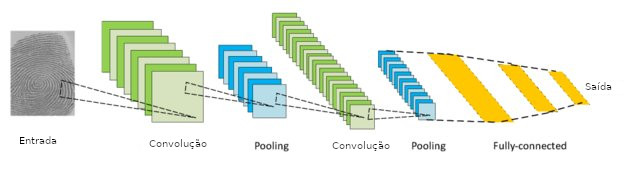
\includegraphics[width=1\linewidth]{recursos/imagens/deep/cnn.jpg}
    \label{cnn:fig:10}

    Fonte: retirada e adaptado de \cite{Minaee2021DeepClassification}.
\end{figure}

Sendo assim, nas próximas seções, fatores que compõem uma rede convolucional serão detalhados, como a camada convolucional (Seção \ref{cnn:conv}), a camada de \textit{pooling} (Seção \ref{cnn:pooling}), fator \textit{dropout} (Seção \ref{cnn:dropout}) e a camada de saída (Seção \ref{cnn:output}) da rede.


\subsection{Camada Convolucional}
\label{cnn:conv}

Quando se trata de CNNs, a modelagem de cada neurônio da camada convolucional conta com um filtro que é aplicado na imagem em questão \cite{ponti2018funciona}, de modo que esses filtros também são compostos por pesos e que a convolução é classificada como uma operação linear \cite{Goodfellow2016}, tendo como resultado o que é definido como \textit{feature maps}.

Além disso, é importante ter ciência de que em meio às camadas convolucionais, há N filtros, os quais são definidos de acordo com o problema em questão e que utilizam dos seus resultados para a formação dos tensores, como é comentado por \cite{ponti2018funciona}.

Uma operação de convolução pode ser retratada por meio da Figura \ref{cnn:fig:6}, em que é  utilizada de uma imagem de entrada (sendo representada pela maior matriz), assim como a definição de um \textit{kernel} de pesos que convolve com a matriz de entrada para extrair características específicas da imagem, sem perder as informações sobre seu arranjo espacial.

\begin{figure}[H]
    \centering
    \caption{Representação do processo de convolução.}
    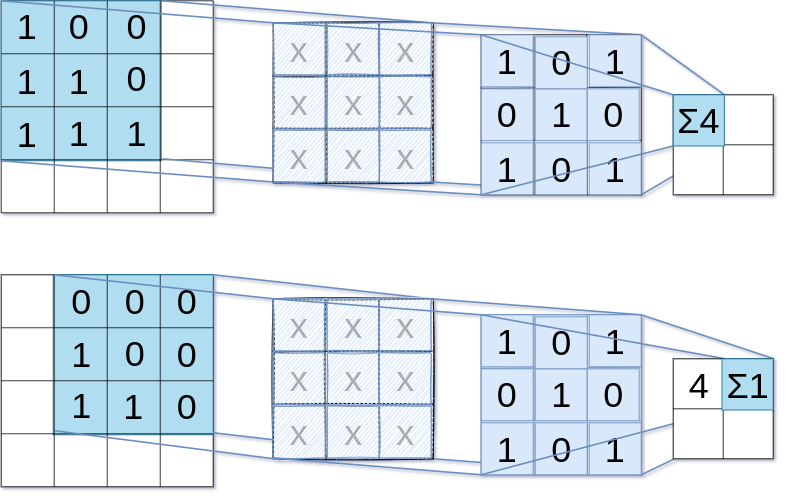
\includegraphics[width=1\linewidth]{recursos/imagens/deep/2d_convolution.png}
    \label{cnn:fig:6}

    Fonte: do próprio autor.
\end{figure}

Ainda na Figura \ref{cnn:fig:6} é possível visualizar que há uma processo de deslizamento do \textit{kernel} para dar continuidade ao processo de convolução que resultará em um dos valores comportados pela saída, processo o qual se repete até a o fim da imagem em ordem de esquerda para a direita, até o fim da linha e de cima para baixo, até o fim das colunas.

Destaca-se que a convolução é um processo de média móvel, ou seja, há o calculo da média ponderada de uma dada janela na imagem, correspondente ao tamanho do \textit{kernel} utilizado, sendo que o \textit{kernel} define os pesos dos respectivos pontos. Por fim, esse \textit{kernel} vai sendo deslizado sobre a imagem, definindo novas janelas na imagem e obtendo suas respectivas médias ponderadas.


\subsection{Camada de \textit{Pooling}}
\label{cnn:pooling}

No âmbito das camadas de \textit{pooling}, vale citar que são amplamente utilizada nas CNNs para reduzir o tempo de treinamento, visto que estas camadas tem como objetivo a redução de dimensionalidade do mapa de características entre as execuções da rede, algo que fica muito claro ao observar a Figura \ref{cnn:fig:7}, que dá forma à técnica conhecida como \textit{max pooling}, a qual captura apenas os maiores valores do mapa de características, de acordo com o deslizamento do \textit{kernel}.

\begin{figure}[H]
    \centering
    \caption{\textit{Max pooling}.}
    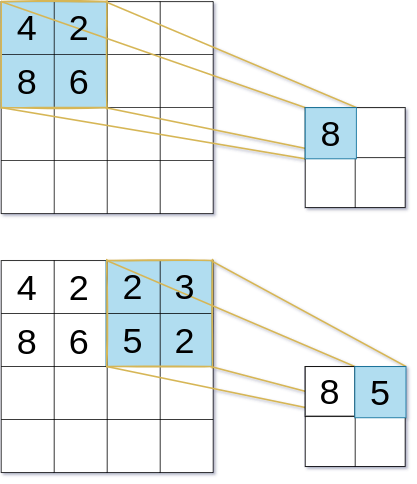
\includegraphics[width=0.5\linewidth]{recursos/imagens/deep/max_pooling.png}
    \label{cnn:fig:7}

    Fonte: do próprio autor.
\end{figure}

\begin{sloppypar}
Ainda, vale mencionar que outros modelos de \textit{pooling} também se fazem presentes na literatura, dos quais podem ser citados o \textit{average pooling}, \textit{median pooling} e \textit{weighted average} \citep{Goodfellow2016} ou até mesmo o \textit{global average pooling}, que reduz o \textit{feature map} em um único valor e é exemplificado por meio da Figura \ref{cnn:fig:8}. Após estes modelos supracitados, a motivação para adaptação do método de \textit{pooling} vem crescendo, de modo que cada modificação contribua para solucionar o problema em questão.
\end{sloppypar}

\begin{figure}[H]
    \centering
    \caption{\textit{Global average pooling}.}
    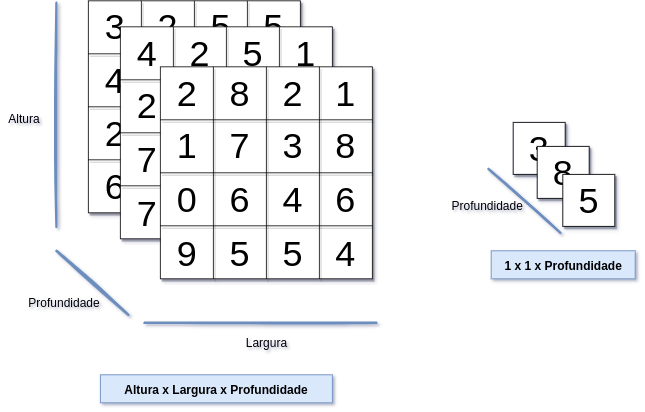
\includegraphics[height=3in]{recursos/imagens/deep/global_average_pooling.png}
    \label{cnn:fig:8}

     Fonte: do próprio autor.
\end{figure}

\subsubsection{\textit{Global Average Pooling}}

\subsubsection{\textit{Average Pooling}}

\subsubsection{\textit{Global Max Pooling}}

\subsubsection{\textit{Max Pooling}}

\subsubsection{\textit{Atrous Spatial Pyramid Pooling}(ASPP)}
\label{cnn:pooling:aspp}
Basicamente, a abordagem relacionada ao módulo de \textit{Atrous Spatial Pyramid Pooling} (ASPP) \citep{Chen2018} está atrelada às segmentações semânticas \citep{Mohan2020}, sendo que este módulo tem como sua principal vantagem a captura de objetos e contexto úteis da imagem em várias escalas diferentes, haja vista que seu comportamento está atrelado à re-amostragem com diversas taxas de convolução para cada \textit{kernel}, possibilitando, assim, a sondagem de um mapa de características, antes mesmo do processo de convolução, com vários campos de visão \cite{Chen2018}. O exemplo desse módulo pode ser visualizado na Figura \ref{proposal:pcapooling:fig:1}.

\begin{figure}[H]
    \centering
    \caption{Exemplo representativo do ASPP.}
    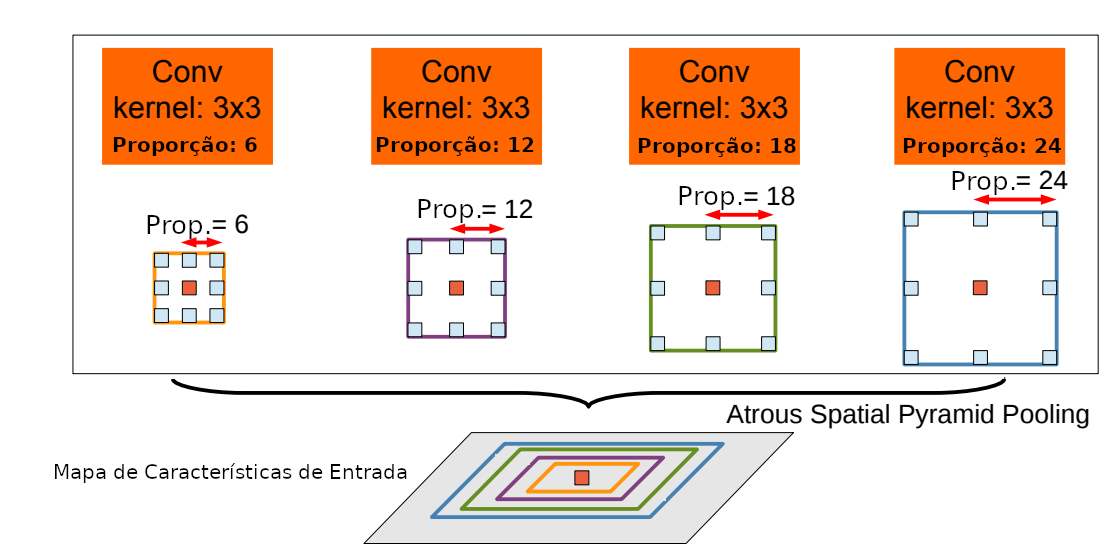
\includegraphics[width=1\textwidth]{recursos/imagens/proposal/aspp.png}
    \label{proposal:pcapooling:fig:1}

    Fonte: retirado e adaptado de \cite{Chen2018}.
\end{figure}

Já quando se trata do módulo de \textit{Pyramid Pooling} \citep{Zhao2017}, vale dizer que este está atrelado à dimensão das características, tendo como principal motivação provar ser um \textit{pooling} de contexto global antes de realizar sua representação \cite{Zhao2017}. Todavia, quando se trata desse modelo de \textit{pooling}, vale dizer que a sua maior vantagem está relacionada à flexibilidade que é cedida às entradas das redes, de modo que torna-se possível realizar entradas com tamanhos variados. O exemplo desse módulo pode ser visualizado na Figura \ref{proposal:pcapooling:fig:2}.

\begin{figure}[H]
    \centering
    \caption{Exemplo representativo do \textit{Pyramid Pooling}.}
    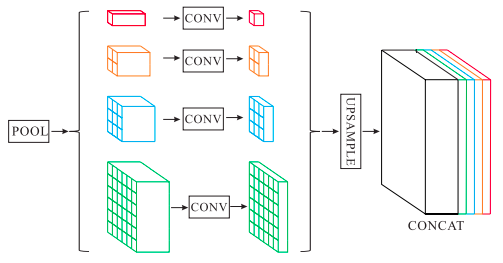
\includegraphics[width=1\textwidth]{recursos/imagens/proposal/pyramidal.png}
    \label{proposal:pcapooling:fig:2}

    Fonte: retirado e adaptado de \cite{Zhao2017}.
\end{figure}

\subsection{\textit{Dropout}}
\label{cnn:dropout}

\begin{sloppypar}
Dentre as técnicas para a prevenção de \textit{overfitting} \cite{Goodfellow2016}, destaca-se a técnica de \textit{dropout} (Seção \ref{cnn:dropout}) que não se aplica na etapa de testes, mas consiste no desligamento aleatório de neurônios de camadas ocultas da rede CNN, de modo que haja uma diminuição do enviesamento de neurônios e eleve a importância dos neurônios restantes.
\end{sloppypar}

Esse processo de \textit{dropout} pode ser representado pela Figura \ref{cnn:fig:9}, demonstrando apenas ligações em neurônios restantes no lado direito.

\begin{figure}[H]
    \centering
    \caption{Processo de \textit{dropout}.}
    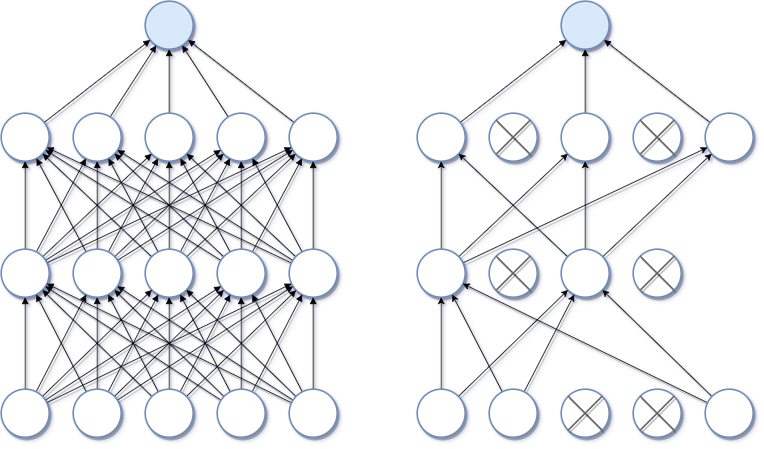
\includegraphics[width=1\linewidth]{recursos/imagens/deep/dropout.png}
    \label{cnn:fig:9}

     Fonte: do próprio autor.
\end{figure}


\subsection{Camada de Saída}
\label{cnn:output}

Após a composição de várias camadas de convolução com filtros e determinadas camadas de \textit{poolling}, os modelos de CNN também contam com uma camada de saída, a qual se faz necessária para a obtenção das classes identificadas na imagem, sendo que essa camada não afeta questões de performance em relação ao tempo de convergência do modelo em questão, além de não afetar o desenvolvimento e evolução da etapa de treinamento.

Por fim, para gerar a saída final normalmente se utiliza de funções de ativação como a Softmax (abordada na Seção \ref{cnn:soft}), possibilitando encontrar a classe de determinado objeto em uma imagem, por exemplo.

\subsection{Transferência de Aprendizado}
\label{cnn:transfer}

\subsection{Aumento de Dados}
\label{cnn:augment}

\subsection{VGG-16}
\label{cnn:vgg}

\subsection{Considerações Finais do Capítulo}